%experimental.tex
\section{Experimental Evaluation: 6-\acs{DOF} \acs{UV} \acs{AID}}
\label{chUV_AID.sec.UVSE3exp}

This Section reports a comparative experimental evaluation of \ac{AID}
and \ac{LS} for the estimation of plant parameters for the
dynamics of a 6-\ac{DOF} \ac{UV}.
% 
We employed the Johns Hopkins University Hydrodynamic Test Facility to
evaluate each parameter identification method's capacity to identify
parameter sets which accurately model \ac{UV} dynamics.
%
The error between the predicted model performance and the
experimentally observed performance is reported as the \ac{MAE}
between the simulated plant roll, pitch, and velocity and the actual
experimental plant roll, pitch, and velocity.
%
Appendices \ref{appenJHUHTF.sec.hydrolab} and \ref{appenJHUHTF.sec.paramEvalMethod}
provide further details about our experimental setup and parameter
evaluation method.


During an experiment, each of the six \ac{JHUROV} \acl{DOF} were
independently excited with either closed-loop control or open-loop
sinusoidal commands. For those \ac{DOF} using closed-loop control, a
sinusoidal reference trajectory was specified to the \ac{JHUROV}
control system. The reference signals for both experiments are given
in Table \ref{chUV_AID.tb.UVSE3expStat}.



\begin{table}[htbp]
\ssp
\caption{Input Specifications for 6-\ac{DOF} \ac{UV} Parameter
  Identification Experiments}  
\begin{center}
\begin{tabular}{cccc}
 \multicolumn{2}{c}{Experiment} & \ac{IDDAT}& \ac{CROSS} \\
\hline
\multicolumn{2}{c}{Experiment Purpose}  & Parameter      &  Parameter \\
              &                         & Identification &  Cross-Validation \\
\hline
\multicolumn{2}{c}{Experiment Run Time} &   31.9 min     &   34.8 min    \\ 
\hline
\ac{DOF}      & {\it Excitation Type} & \multicolumn{2}{c}{\it Closed Loop Trajectory-Tracking} \\
world x  &  Cos Frequency  & 0.185 rad/sec & 0.242 rad/sec \\ 
         &  Cos Amplitude  &    0.60 m     &     0.60 m    \\ 
\hline
\ac{DOF}      & {\it Excitation Type} & \multicolumn{2}{c}{\it Closed Loop Trajectory-Tracking} \\
world y  &  Cos Frequency  & 0.286 rad/sec & 0.210 rad/sec \\ 
         &  Cos Amplitude  &    0.60 m     &     0.60 m    \\ 
\hline
\ac{DOF}      & {\it Excitation Type} & \multicolumn{2}{c}{\it Closed Loop Trajectory-Tracking} \\
world z  &  Cos Frequency  & 0.242 rad/sec & 0.185 rad/sec \\ 
         &  Cos Amplitude  &    0.50 m     &     0.50 m    \\ 
\hline
Torque   & {\it Excitation Type} & \multicolumn{2}{c}{\it Open Loop Torque Input} \\
about \ac{DOF}&  Cos Frequency  & 0.262 rad/sec & 0.224 rad/sec \\ 
body x   &  Cos Amplitude  &    40 N m    &     40 N m     \\ 
\hline
Torque   & {\it Excitation Type} & \multicolumn{2}{c}{\it Open Loop Torque Input} \\
about \ac{DOF}&  Cos Frequency  & 0.449 rad/sec & 0.331 rad/sec \\ 
body y   &  Cos Amplitude  &    55 N m    &     55 N m     \\ 
\hline
\ac{DOF}      & {\it Excitation Type} & \multicolumn{2}{c}{\it Closed Loop Trajectory-Tracking} \\
heading  &  Cos Frequency  & 0.210 rad/sec & 0.286 rad/sec \\ 
         &  Cos Amplitude  &    45$^\circ$  &   45$^\circ$   \\ 
\hline \end{tabular}
\end{center}
\label{chUV_AID.tb.UVSE3expStat}
\end{table}



\ac{AID} was implemented as a discrete time approximation of the
continuous time algorithm.  
%
%Once every 100ms the most recent state measurements, commanded
%torque, commanded force, parameter estimates, and velocity
%estimates were used to calculate the velocity and parameter
%estimate derivatives
%(\ref{chUV_AID.eq.UV_SE3_Estimator})-(\ref{chUV_AID.eq.UV_SE3_BuoyId}).
%
Euler integration of
(\ref{chUV_AID.eq.UV_SE3_Estimator})-(\ref{chUV_AID.eq.UV_SE3_BuoyId})
for 100ms time steps
provided the time series of parameter and angular velocity
estimates.
%
100ms is one to two orders-of-magnitude smaller than the state signal
variation rates of 1 second or greater observed during quasi-periodic
\ac{JHUROV} operations.
%
The experiments were designed to generate thruster commands varying
slowly enough to admit the use of steady state thruster models.
%
In practice, first-order Euler integration provided performance
similar to the 4th-order integration implemented in simulation.


The \ac{AID} algorithm was initialized with the measured angular
position, measured angular velocity, measured translational velocity,
and \acf{INITP} in Tables \ref{chUV_AID.tb.UVSE3_INIT_massGravParam}
and \ref{chUV_AID.tb.UVSE3_INIT_dragParam}.
%
%Note that the \ac{INITP} was chosen such that each scalar
%parameter was within an order-of-magnitude of the value to be identified.
%
Based on our previous studies with second-order rigid body adaptive
identification algorithms (Sections \ref{chSMS_ID.sec.SO3_AID_Sim} and
\ref{chUV_AID.sec.UVSO3exp}), we chose adaption gains of $a=10$,
$\gamma_1=5000$, $\gamma_2=20000$, $\gamma_3=2000$, and
$\gamma_4=2000$.


\begin{table}[htbp]
\ssp
\caption{\ac{UV} mass and gravitational parameter values used to initialize \ac{AID}.}
\begin{center}
\begin{tabular}{c|c}
Parameter Symbol & \ac{INITP} Values \\ \hline
$\hat{M}(t_0)$ & $ \left[\begin{array}{cccccc} 100.0 & 0 & 0 & 0 & 0 & 0\\ 0 & 100.0 & 0 & 0 & 0 & 0\\ 0 & 0 & 100.0 & 0 & 0 & 0\\ 0 & 0 & 0 & 100.0 & 0 & 0\\ 0 & 0 & 0 & 0 & 100.0 & 0\\ 0 & 0 & 0 & 0 & 0 & 100.0 \end{array}\right] $ \\ 
$\hat{g}(t_0)$ & 0.0 \\ 
$\hat{b}(t_0)$ & $ \left[\begin{array}{c} 0\\ 0\\ 100.0 \end{array}\right] $ \\ 
\end{tabular}
\end{center}
\label{chUV_AID.tb.UVSE3_INIT_massGravParam}
\end{table}


\begin{table}[htbp]
\ssp
\caption{The \ac{UV} drag parameter values used to initialize \ac{AID}.}
\begin{center}
\begin{tabular}{c|c}
Parameter Symbol & \ac{INITP} Values \\ \hline
$\hat{D}_1(t_0)$ & $ \left[\begin{array}{cccccc} -100.0 & 0 & 0 & 0 & 0 & 0\\ 0 & -100.0 & 0 & 0 & 0 & 0\\ 0 & 0 & -100.0 & 0 & 0 & 0\\ 0 & 0 & 0 & -100.0 & 0 & 0\\ 0 & 0 & 0 & 0 & -100.0 & 0\\ 0 & 0 & 0 & 0 & 0 & -100.0 \end{array}\right] $ \\ 
$\hat{D}_2(t_0)$ & $ \left[\begin{array}{cccccc} -100.0 & 0 & 0 & 0 & 0 & 0\\ 0 & -100.0 & 0 & 0 & 0 & 0\\ 0 & 0 & -100.0 & 0 & 0 & 0\\ 0 & 0 & 0 & -100.0 & 0 & 0\\ 0 & 0 & 0 & 0 & -100.0 & 0\\ 0 & 0 & 0 & 0 & 0 & -100.0 \end{array}\right] $ \\ 
$\hat{D}_3(t_0)$ & $ \left[\begin{array}{cccccc} -100.0 & 0 & 0 & 0 & 0 & 0\\ 0 & -100.0 & 0 & 0 & 0 & 0\\ 0 & 0 & -100.0 & 0 & 0 & 0\\ 0 & 0 & 0 & -100.0 & 0 & 0\\ 0 & 0 & 0 & 0 & -100.0 & 0\\ 0 & 0 & 0 & 0 & 0 & -100.0 \end{array}\right] $ \\ 
$\hat{D}_4(t_0)$ & $ \left[\begin{array}{cccccc} -100.0 & 0 & 0 & 0 & 0 & 0\\ 0 & -100.0 & 0 & 0 & 0 & 0\\ 0 & 0 & -100.0 & 0 & 0 & 0\\ 0 & 0 & 0 & -100.0 & 0 & 0\\ 0 & 0 & 0 & 0 & -100.0 & 0\\ 0 & 0 & 0 & 0 & 0 & -100.0 \end{array}\right] $ \\ 
$\hat{D}_5(t_0)$ & $ \left[\begin{array}{cccccc} -100.0 & 0 & 0 & 0 & 0 & 0\\ 0 & -100.0 & 0 & 0 & 0 & 0\\ 0 & 0 & -100.0 & 0 & 0 & 0\\ 0 & 0 & 0 & -100.0 & 0 & 0\\ 0 & 0 & 0 & 0 & -100.0 & 0\\ 0 & 0 & 0 & 0 & 0 & -100.0 \end{array}\right] $ \\ 
$\hat{D}_6(t_0)$ & $ \left[\begin{array}{cccccc} -100.0 & 0 & 0 & 0 & 0 & 0\\ 0 & -100.0 & 0 & 0 & 0 & 0\\ 0 & 0 & -100.0 & 0 & 0 & 0\\ 0 & 0 & 0 & -100.0 & 0 & 0\\ 0 & 0 & 0 & 0 & -100.0 & 0\\ 0 & 0 & 0 & 0 & 0 & -100.0 \end{array}\right] $ \\ 
\end{tabular}
\end{center}
\label{chUV_AID.tb.UVSE3_INIT_dragParam}
\end{table}


\subsection{Experimental Results}%\label{ref.expResults}

\begin{table}[htbp]
\ssp
\caption{The \ac{UV} mass and gravitational parameters identified
  using \ac{AID} and the \ac{IDDAT} dataset.}
\begin{center}
\begin{tabular}{c|c}
Parameter Symbol & \ac{AIDP} Values \\ \hline
$\hat{M}(t_f)$ & $ \left[\begin{array}{cccccc} 996.9 & -6.166 & 9.118 & 53.64 & -76.78 & 111.7\\ -6.166 & 1275.0 & 14.23 & -56.45 & 41.07 & -43.3\\ 9.118 & 14.23 & 1378.0 & -17.57 & 69.42 & 43.95\\ 53.64 & -56.45 & -17.57 & 308.7 & 21.87 & 39.99\\ -76.78 & 41.07 & 69.42 & 21.87 & 322.3 & -48.32\\ 111.7 & -43.3 & 43.95 & 39.99 & -48.32 & 467.4 \end{array}\right] $ \\ 
$\hat{g}(t_f)$ & -21.77 \\ 
$\hat{b}(t_f)$ & $ \left[\begin{array}{c} 5.966\\ -0.9802\\ 342.8 \end{array}\right] $ \\ 
\end{tabular}
\end{center}
\label{chUV_AID.tb.UVSE3_AID_massGravParam}
\end{table}


\begin{table}[htbp]
\ssp
\caption{The \ac{UV} drag parameters identified using \ac{AID} and the
  \ac{IDDAT} data.}
\begin{center}
\begin{tabular}{c|c}
Parameter Symbol & \ac{AIDP} Values \\ \hline
$\hat{D}_1(t_f)$ & $ \left[\begin{array}{cccccc} -466.7 & 4.902 & -14.54 & -19.92 & -0.3734 & -3.236\\ 71.43 & -331.6 & -27.36 & 119.8 & -13.05 & 12.08\\ -67.64 & -1.584 & -528.8 & -11.23 & 42.6 & -22.18\\ 0.03723 & -12.6 & 97.29 & -270.7 & 19.31 & -56.57\\ 17.39 & -14.41 & -47.56 & -19.17 & -51.29 & 6.865\\ -36.24 & 5.508 & -3.391 & 44.59 & -13.47 & -155.7 \end{array}\right] $ \\ 
$\hat{D}_2(t_f)$ & $ \left[\begin{array}{cccccc} -342.9 & 15.59 & 35.52 & -19.45 & -30.78 & -27.73\\ -16.96 & -618.6 & 68.14 & 107.7 & -37.52 & 42.93\\ 7.135 & 19.27 & -578.9 & 19.15 & 49.08 & -21.97\\ -11.15 & 49.91 & 69.85 & -279.2 & 30.13 & -19.8\\ 52.72 & -63.28 & -11.81 & -22.2 & -42.57 & 38.04\\ -31.44 & 43.94 & -40.48 & 77.72 & -16.38 & -150.4 \end{array}\right] $ \\ 
$\hat{D}_3(t_f)$ & $ \left[\begin{array}{cccccc} -373.0 & 9.072 & 43.92 & -9.852 & -26.69 & 7.863\\ -12.09 & -466.7 & 6.452 & 138.2 & -11.46 & 67.43\\ -31.76 & 52.37 & -685.6 & -1.646 & 20.42 & -2.191\\ -21.4 & 3.283 & 146.3 & -261.8 & 32.96 & -33.43\\ 4.241 & -32.42 & -17.53 & -30.22 & -56.54 & -11.55\\ -45.66 & 24.02 & -38.2 & 40.72 & -28.91 & -241.1 \end{array}\right] $ \\ 
$\hat{D}_4(t_f)$ & $ \left[\begin{array}{cccccc} -292.8 & -10.59 & 35.93 & -8.17 & -18.11 & -25.44\\ 4.436 & -342.0 & 13.63 & 190.4 & -3.024 & 45.74\\ 9.531 & -6.416 & -362.0 & -19.08 & 23.41 & -14.81\\ 2.579 & 32.18 & 62.65 & -207.2 & 16.85 & 2.63\\ 4.186 & -6.082 & -7.507 & -22.97 & -73.4 & 5.957\\ 3.196 & 20.58 & 1.016 & 62.8 & -19.93 & -142.3 \end{array}\right] $ \\ 
$\hat{D}_5(t_f)$ & $ \left[\begin{array}{cccccc} -212.3 & -16.1 & 7.133 & -15.9 & -21.23 & -4.932\\ 19.71 & -242.1 & -6.173 & 44.77 & -7.459 & 19.94\\ -9.7 & -17.81 & -248.4 & 0.08174 & 32.39 & -5.403\\ -2.604 & 11.03 & 39.88 & -162.8 & 24.41 & -9.847\\ 4.528 & -3.59 & -16.11 & -10.59 & -66.71 & 17.56\\ -11.06 & -4.563 & 0.2745 & 19.88 & -14.07 & -148.7 \end{array}\right] $ \\ 
$\hat{D}_6(t_f)$ & $ \left[\begin{array}{cccccc} -398.9 & -8.592 & -25.27 & -11.01 & -43.3 & -25.29\\ -53.06 & -602.1 & 24.9 & 133.0 & -28.92 & 70.24\\ 4.612 & -16.02 & -582.0 & -0.02913 & 77.21 & -53.36\\ -3.501 & 13.71 & 115.5 & -283.3 & 25.63 & -153.0\\ 11.5 & -44.13 & -35.11 & -25.37 & -41.52 & -18.43\\ -57.68 & 33.12 & -49.59 & 76.05 & -17.43 & -109.2 \end{array}\right] $ \\ 
\end{tabular}
\end{center}
\label{chUV_AID.tb.UVSE3_AID_dragParam}
\end{table}



\begin{table}[htbp]
\ssp
\caption{The \ac{UV} mass and gravitational parameters identified
  using \ac{LS} and the \ac{IDDAT} dataset.}
\begin{center}
\begin{tabular}{c|c}
Parameter Symbol & \ac{LSP} Values \\ \hline
$\hat{M}(t_f)$ & $ \left[\begin{array}{cccccc} 446.7 & 13.29 & 35.18 & 20.74 & -27.2 & 37.66\\ 13.29 & 669.5 & -0.2402 & -14.65 & 2.878 & -21.9\\ 35.18 & -0.2402 & 896.2 & -16.36 & 11.14 & 35.23\\ 20.74 & -14.65 & -16.36 & 39.53 & -7.008 & 17.43\\ -27.2 & 2.878 & 11.14 & -7.008 & 65.47 & -2.574\\ 37.66 & -21.9 & 35.23 & 17.43 & -2.574 & 116.8 \end{array}\right] $ \\ 
$\hat{g}(t_f)$ & -19.7 \\ 
$\hat{b}(t_f)$ & $ \left[\begin{array}{c} 0.7842\\ 6.807\\ 279.8 \end{array}\right] $ \\ 
\end{tabular}
\end{center}
\label{chUV_AID.tb.UVSE3_LS_massGravParam}
\end{table}


\begin{table}[htbp]
\ssp
\caption{The \ac{UV} drag parameters identified using \ac{LS} and the
  \ac{IDDAT} dataset.}
\begin{center}
\begin{tabular}{c|c}
Parameter Symbol & \ac{LSP} Values \\ \hline
$\hat{D}_1(t_f)$ & $ \left[\begin{array}{cccccc} -640.7 & 29.14 & -77.14 & -206.0 & 399.7 & -57.4\\ 426.7 & -146.6 & -191.1 & -53.18 & 310.4 & -242.6\\ 50.05 & -65.4 & -1078.0 & 216.5 & 32.88 & -108.7\\ -2.037 & 35.94 & 4.818 & -557.7 & -19.11 & 58.69\\ 60.09 & 65.24 & -2.878 & 78.19 & -108.7 & 74.52\\ -32.74 & 15.27 & -19.89 & -77.99 & 81.52 & -82.61 \end{array}\right] $ \\ 
$\hat{D}_2(t_f)$ & $ \left[\begin{array}{cccccc} -416.7 & -54.12 & 88.38 & -53.97 & -79.78 & -63.98\\ -20.42 & -575.1 & 101.8 & -75.27 & -260.0 & 67.67\\ -25.36 & -75.01 & -979.1 & 429.8 & -130.5 & -45.88\\ -37.62 & 69.31 & 0.004228 & -318.2 & 73.01 & 16.12\\ 52.75 & -31.51 & -40.18 & -32.51 & -183.8 & 10.49\\ -62.16 & -15.68 & -89.55 & 33.62 & 243.3 & -220.9 \end{array}\right] $ \\ 
$\hat{D}_3(t_f)$ & $ \left[\begin{array}{cccccc} -894.2 & 293.0 & 42.96 & -203.4 & -424.3 & 15.49\\ -115.2 & -1247.0 & -215.0 & 164.9 & 283.9 & 131.6\\ -120.7 & 165.4 & -901.3 & 72.91 & -150.7 & 168.2\\ -25.58 & 84.36 & 195.6 & -318.2 & -40.94 & 26.2\\ 145.6 & -164.2 & -46.79 & 73.39 & -321.2 & 27.31\\ -115.2 & 164.7 & -143.7 & -67.74 & -72.01 & -514.8 \end{array}\right] $ \\ 
$\hat{D}_4(t_f)$ & $ \left[\begin{array}{cccccc} -22.32 & -55.78 & 266.5 & 233.5 & -737.6 & 258.0\\ -445.6 & -242.8 & 463.0 & 1680.0 & 255.3 & -128.4\\ 61.74 & -83.5 & -454.2 & -943.5 & -53.48 & -144.2\\ 45.38 & 149.0 & -167.4 & 235.8 & -10.58 & 40.72\\ 89.95 & -16.57 & -114.2 & -32.4 & -58.5 & -80.68\\ -39.36 & -14.35 & 135.3 & 278.7 & -508.8 & -114.7 \end{array}\right] $ \\ 
$\hat{D}_5(t_f)$ & $ \left[\begin{array}{cccccc} -541.9 & -201.2 & -218.5 & -4.108 & -1155.0 & 338.4\\ 802.6 & -1098.0 & -648.5 & -353.1 & -46.14 & -232.1\\ 123.8 & -116.6 & -1045.0 & 209.3 & -203.8 & -111.9\\ -81.21 & 59.62 & 6.686 & -450.4 & 90.86 & 44.2\\ 11.35 & 45.01 & 96.38 & -126.6 & 216.3 & 41.87\\ -41.39 & -1.279 & 223.2 & -8.406 & -221.2 & -42.09 \end{array}\right] $ \\ 
$\hat{D}_6(t_f)$ & $ \left[\begin{array}{cccccc} -310.2 & 98.97 & -39.83 & 86.85 & 22.8 & -142.3\\ -172.0 & -730.8 & 113.5 & 166.2 & -560.2 & 266.3\\ 1.31 & -43.02 & -536.0 & 166.4 & 370.4 & 68.14\\ -22.85 & 1.085 & 16.88 & -247.2 & -57.23 & -76.39\\ -28.74 & -68.49 & -109.2 & 28.06 & -310.4 & 17.32\\ -155.9 & 21.63 & -77.06 & -27.19 & 40.62 & -24.28 \end{array}\right] $ \\ 
\end{tabular}
\end{center}
\label{chUV_AID.tb.UVSE3_LS_dragParam}
\end{table}


The \ac{IDDAT} dataset was used to identify plant parameters of the
6-\ac{DOF} plant model (\ref{chModels.eq.UVSE3plant}) with both the
adaptive identification and least squares algorithms.
%
\Cref{chUV_AID.tb.UVSE3_AID_massGravParam,chUV_AID.tb.UVSE3_AID_dragParam}
report the \acf{AIDP} estimated using  6-\ac{DOF} \ac{UV} \ac{AID} (as
per Section \ref{chUV_AID.sec.UV_SE3_AID}).
%
\Cref{chUV_AID.tb.UVSE3_LS_massGravParam,chUV_AID.tb.UVSE3_LS_dragParam}
report the \acf{LSP}  estimated using 6-\ac{DOF} \ac{UV} \ac{LS} (as
per Section \ref{chUV_AID.sec.leastSquares}).
%
The parameter sets \ac{AIDP}, \ac{LSP}, and \ac{INITP} were used as
 parameter sets for three 6-\ac{DOF} \ac{UV} models;
the \acf{AIDPM}, the \acf{LSPM}, and the \acf{INITPM}.


Using the force and torque inputs from the \ac{CROSS} dataset,
\Cref{chUV_AID.fig.SE3_crossPos,chUV_AID.fig.SE3_crossBodVel,chUV_AID.fig.SE3_crossAngVel}
compare the states from simulations of \ac{AIDPM},
\ac{LSPM}, and \ac{INITPM} to the measured \ac{JHUROV} states from
the \ac{CROSS} dataset.
%
Each of these Figures display three minute subsets of 30 minutes of
state data generated by driving simulations of \ac{AIDPM},
\ac{LSPM}, and \ac{INITPM} using the torque data from the \ac{CROSS}
dataset.
%
Similar simulations of \ac{AIDPM}, \ac{LSPM}, and \ac{INITPM} were
created using the force and torque commands from the \ac{IDDAT} dataset.
%
\Cref{chUV_AID.tb.SE3_pos_MAE,chUV_AID.tb.SE3_vel_MAE} summarize the \ac{MAE} between
measured and simulated vehicle state for each experimental dataset,
6-\ac{DOF} \ac{UV} model, 
and open-loop-stable \ac{DOF}.


%changes after matlab generate MAE table:
% 1)split this table into two tables, 
% 2) moved "paramter set" onto two table rows,
% 3)added the over-labels for velocites, 
% 4)changed the first couple words of both captions
% 5)added '0' to numeric values where sigificant figure rules required it
% 6)changed table labels 

\begin{table}[htbp]
\ssp
\caption{\acfp{MAE} between measured and simulated angular position states for  
  all pairs of 6-\ac{DOF} \ac{UV} experiments and 6-\ac{DOF} \ac{UV} models.}
\begin{center}
\begin{tabular}{p{1.75cm}|ccc}
 \ac{UV}    &          &     &      \\
  Model     & Experiment & Rol & Pit  \\ \hline
\ac{AIDPM} & \ac{CROSS} & 2$^\circ$ & 2.1$^\circ$  \\
\ac{LSPM} & \ac{CROSS} & 1.38$^\circ$ & 1.65$^\circ$  \\
\ac{INITPM} & \ac{CROSS} & 9.9$^\circ$ & 15.0$^\circ$  \\
\ac{AIDPM} & \ac{IDDAT} & 1.96$^\circ$ & 2.3$^\circ$  \\
\ac{LSPM} & \ac{IDDAT} & 1.30$^\circ$ & 1.50$^\circ$  \\
\ac{INITPM} & \ac{IDDAT} & 10.0$^\circ$ & 15.2$^\circ$  \\
\end{tabular}
\end{center}
\label{chUV_AID.tb.SE3_pos_MAE}
\end{table}
%

\begin{table}[htbp]
\ssp
\caption{\acfp{MAE} between simulated and measured velocity states for  
  all pairs of 6-\ac{DOF} \ac{UV} experiments and 6-\ac{DOF} \ac{UV} models.}
\begin{center}
\begin{tabular}{p{1.5cm}|ccccccc}
\ac{UV}  &  & \multicolumn{3}{c}{Translational Velocity} & \multicolumn{3}{c}{Angular Velocity} \\
 Model & Exp  & BodVelX & BodVelY & BodVelZ & AngVelX & AngVelY & AngVelZ \\ \hline
\ac{AIDPM} & \ac{CROSS}  & 0.062m/s & 0.058m/s & 0.037m/s & 1.39$^\circ$/s & 1.35$^\circ$/s & 5.0$^\circ$/s \\
\ac{LSPM} & \ac{CROSS}  & 0.050m/s & 0.052m/s & 0.024m/s & 1.38$^\circ$/s & 1.39$^\circ$/s & 6.3$^\circ$/s \\
\ac{INITPM} & \ac{CROSS}  & 0.165m/s & 0.26m/s & 0.25m/s & 5.1$^\circ$/s & 3.3$^\circ$/s & 3.9$^\circ$/s \\
\ac{AIDPM} & \ac{IDDAT}  & 0.061m/s & 0.06m/s & 0.039m/s & 1.62$^\circ$/s & 1.43$^\circ$/s & 3.4$^\circ$/s \\
\ac{LSPM} & \ac{IDDAT}  & 0.045m/s & 0.048m/s & 0.026m/s & 1.58$^\circ$/s & 1.25$^\circ$/s & 4.1$^\circ$/s \\
\ac{INITPM} & \ac{IDDAT}  & 0.156m/s & 0.27m/s & 0.29m/s & 6.8$^\circ$/s & 3.4$^\circ$/s & 3.8$^\circ$/s \\
\end{tabular}
\end{center}
\label{chUV_AID.tb.SE3_vel_MAE}
\end{table}




\begin{center}
\begin{figure}[htbp]
  \begin{center}
    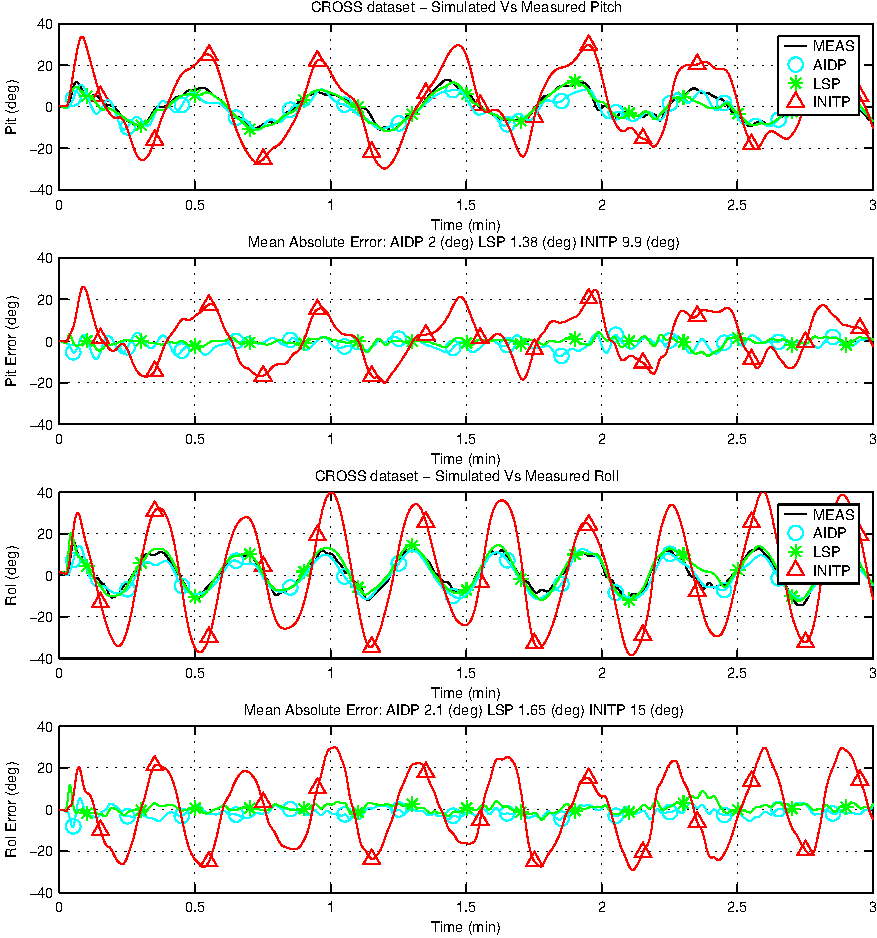
\includegraphics[width=6in]{./chUV_AID/images/SE3_crossPos}
  \end{center}
  \caption{ Representative data of experimental and simulated
    \ac{JHUROV} states for the \ac{CROSS} dataset. In the pitch and
    roll plots, the measured state is plotted together with the
    simulation state from three model simulations. The states from
    \ac{AIDPM} are plotted in blue and marked with circles.  The
    states from \ac{LSPM} are plotted in green and marked with stars.
    The states from \ac{INITPM} are plotted in red and marked with
    triangles.  For each \ac{DOF}, the error between the measured
    positions and their estimates is shown.  }
  \label{chUV_AID.fig.SE3_crossPos}
\end{figure}
\end{center}


\begin{center}
\begin{figure}[htbp]
  \begin{center}
    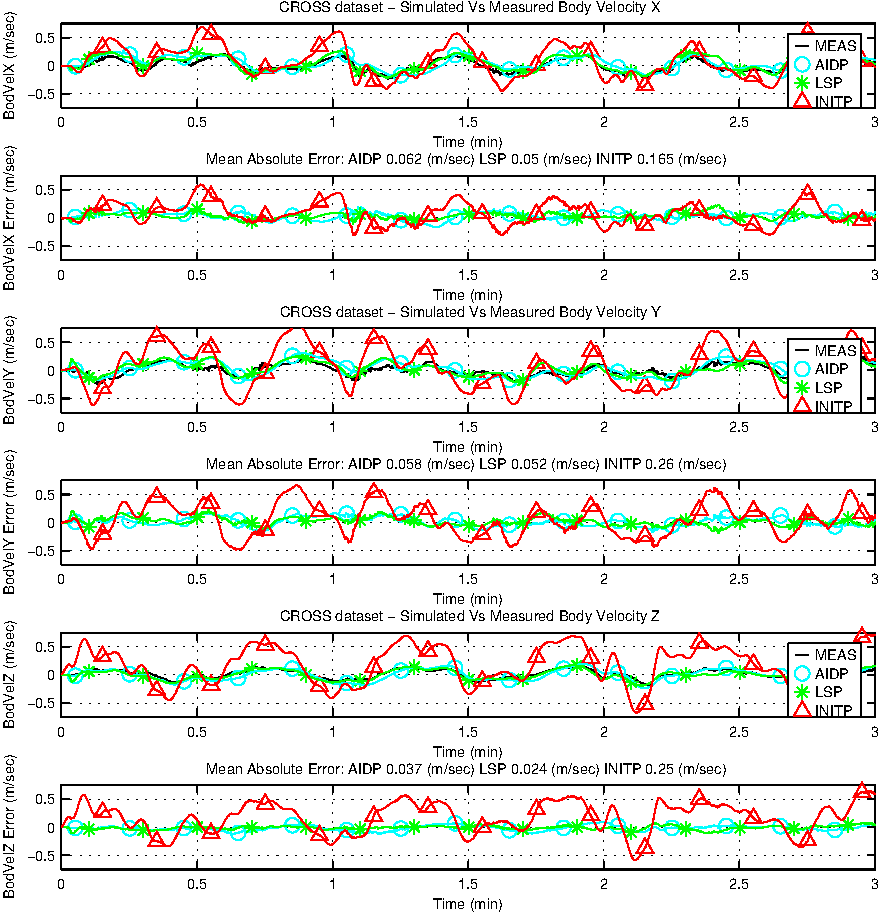
\includegraphics[width=6in]{./chUV_AID/images/SE3_crossBodVel}
  \end{center}
  \caption{
    Representative data of experimental and simulated
    \ac{JHUROV} states for the \ac{CROSS} dataset. In the x, y and z
    body velocity, the measured state is plotted together with the
    simulation state from three model simulations. The states from
    \ac{AIDPM} are plotted in blue and marked with circles.  The
    states from \ac{LSPM} are plotted in green and marked with stars.
    The states from \ac{INITPM} are plotted in red and marked with
    triangles.  For each \ac{DOF}, the error between the measured
    positions and their estimates is shown. 
  }
  \label{chUV_AID.fig.SE3_crossBodVel}
\end{figure}
\end{center}



\begin{center}
\begin{figure}[htbp]
  \begin{center}
    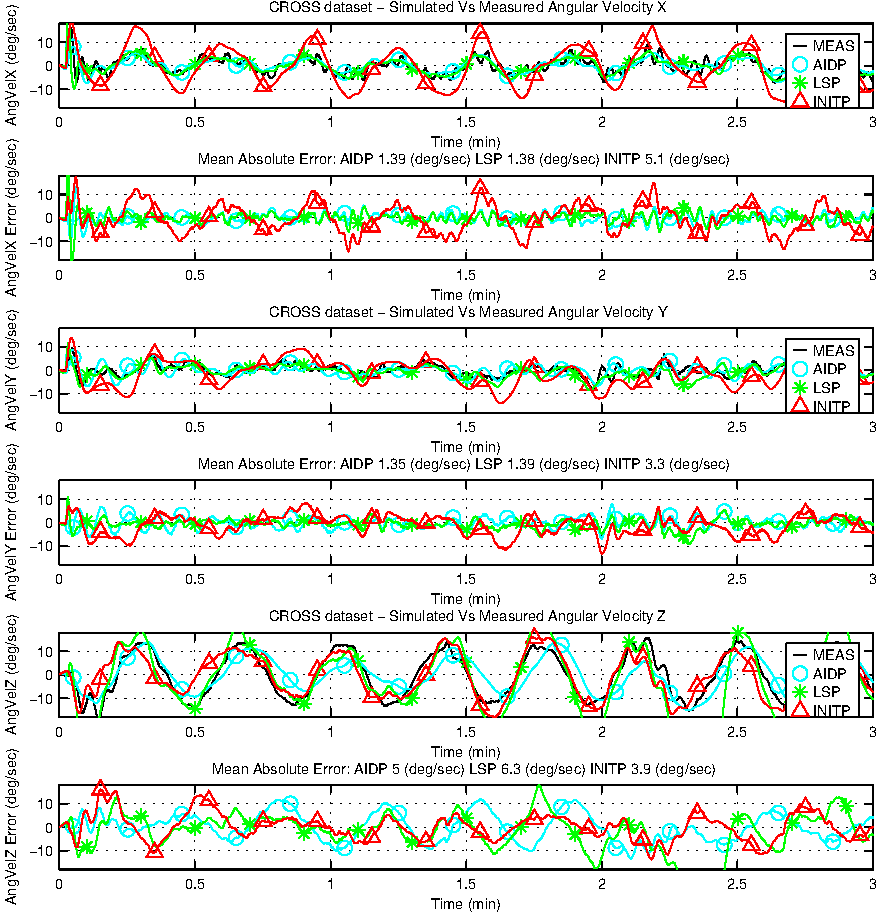
\includegraphics[width=6in]{./chUV_AID/images/SE3_crossAngVel}
  \end{center}
  \caption{ Representative data of experimental and simulated
    \ac{JHUROV} states for the \ac{CROSS} dataset. In the x, y and z
    angular velocity plots, the measured state is plotted together
    with the simulation state from three model simulations. The states
    from \ac{AIDPM} are plotted in blue and marked with circles.  The
    states from \ac{LSPM} are plotted in green and marked with stars.
    The states from \ac{INITPM} are plotted in red and marked with
    triangles.  For each \ac{DOF}, the error between the measured
    positions and their estimates is shown.}
  \label{chUV_AID.fig.SE3_crossAngVel}
\end{figure}
\end{center}


\subsection{Analysis of Experimental Results}


\Cref{chUV_AID.fig.SE3_crossPos,chUV_AID.fig.SE3_crossBodVel,chUV_AID.fig.SE3_crossAngVel}
reveal that the ability of a simulated plant model to match
experimentally observed plant performance is dependent on the model's
plant parameters.
%
Comparing the states produced by simulating \ac{AIDPM} and \ac{LSPM}
with those from \ac{INITPM} (a model which uses the arbitrarily chosen
\ac{INITP} parameter set), we see that both experimentally identified
models are better at matching experimentally observed dynamic plant
behavior.
%
Tables \ref{chUV_AID.tb.SE3_pos_MAE} and \ref{chUV_AID.tb.SE3_vel_MAE}
confirm that the \ac{AIDPM} and \ac{LSPM} match \ac{JHUROV} performance
better than the \ac{INITPM}.

Tables \ref{chUV_AID.tb.SE3_pos_MAE} and
\ref{chUV_AID.tb.SE3_vel_MAE} suggest that both identified models provide
similar \ac{MAE} values for the \ac{IDDAT} dataset.
%
However, since this experiment was used to identify both models, the
question arises ``How will each model reproduce vehicle performance
for experiments not used for model identification?''  
%
The rest of this discussion addresses this important question, 
focusing on which (if any) of the  identified models are better at matching
\ac{JHUROV} performance in cross-validation (as per Appendix \ref{appenJHUHTF.sec.paramEvalMethod}).
%
\ac{MAE} values from comparing simulated and measured states for the
\ac{CROSS} dataset show that modeling the \ac{JHUROV} using the \acf{LSPM}
is marginally better than modeling the \ac{JHUROV} using the \acf{AIDPM},
as seen in the angular position \acp{MAE} in Table
\ref{chUV_AID.tb.SE3_pos_MAE} and translational velocity \acp{MAE} in
Table \ref{chUV_AID.tb.SE3_vel_MAE}.
%
Both Figure \ref{chUV_AID.fig.SE3_crossAngVel} and Table
\ref{chUV_AID.tb.SE3_vel_MAE} indicate that the \ac{AIDPM} and
\ac{LSPM} provide a similar capacity to estimate the \ac{JHUROV}'s
angular velocity.
%
In
\Cref{chUV_AID.fig.SE3_crossPos,chUV_AID.fig.SE3_crossBodVel,chUV_AID.fig.SE3_crossAngVel}
the \ac{LSPM} and \ac{AIDPM} accurately reproduce the experimentally
observed states, failing only to reproduce the very highest frequency
fluctuations observed experimentally (such as those seen in the x
angular velocity subplots of Figure
\ref{chUV_AID.fig.SE3_crossAngVel}).
%
Taken together
\Cref{chUV_AID.fig.SE3_crossPos,chUV_AID.fig.SE3_crossBodVel,chUV_AID.fig.SE3_crossAngVel}
and \Cref{chUV_AID.tb.SE3_pos_MAE,chUV_AID.tb.SE3_vel_MAE} indicate
that the character of \ac{JHUROV} performance is captured well by both
the \ac{LSPM} and \ac{AIDPM}.



%-------------------------------------------------------------------
% Figure \ref{fig.crossAll} shows that the ability for a simulated model
% plant to match experimentally observed plant performance is dependent
% on the model plant parameters.
% %
% Comparing the AID and LS parameter sets with the arbitrarily chosen
% INIT parameter set, the two experimentally identified parameter sets
% provide much better estimates of the vehicle's states.
% %
% Table \ref{tb.MAE} confirms that the AID and LS parameter sets are
% better than the INIT parameter set at modeling \ac{JHUROV} performance.
% %
% Considering the LS and AID model performance for IDDAT, the LS model
% is better at matching the measured vehicle states.
% %
% However, using the same dataset to both create and evaluate a model
% can be a poor predictor of model performance for other inputs.
% %
% Therefore we have performed the cross-validation experiment CROSS.
% %
% Note that all three models provide similar MAE values for both the
% IDDAT and CROSS datasets, an indication that each model will provide
% similar predictive accuracy across the class of inputs physically
% possible for \ac{JHUROV} operation.


% The cross-validation shows that the LS model is better at matching the
% measured vehicle states than the AID model, especially in the angular
% position and linear velocity \ac{DOF}s.
% %
% Table \ref{tb.MAE} indicates that both models provide a similar
% capacity to estimate the \ac{JHUROV}'s angular velocity, which can be seen
% in the Figure \ref{fig.crossAll} y angular velocity plots.
% %
% Here note the complex trajectory the \ac{JHUROV} is following in angular
% velocity.
% %
% Both the LS and AID models are following the general direction of JHU
% ROV angular accelerations with most of the modeling error coming from
% an inability to model the finer details.
% %
% The example plots for two other \ac{DOF} (roll and body
% velocity z) in Figure \ref{fig.crossAll} show the \ac{JHUROV} following
% simpler trajectories.  
% %
% In the roll and body velocity z \ac{DOF}s the LS and AID models are closely
% following the measured \ac{JHUROV} states.
% %
% However, in both \ac{DOF}, specific times can be seen where the AID model
% states are slightly larger offset from measured states.
% %
% Taken together, Figure \ref{fig.crossAll} and Table \ref{tb.MAE}
% indicate that the LS model is marginally better at matching measured
% vehicle performance, but the character of \ac{JHUROV} performance is well
% captured by both identified models.
